\input{ieee-preamble}
\usepackage{graphicx}
\hypersetup{
  pdftitle={Delta Robot with Damped Articulations},
  pdfauthor={Santiago Restrepo},
  pdfsubject={Technical summary of the 2017 undergraduate thesis},
  pdfkeywords={Delta robot, parallel manipulator, compliant mechanism,
    constrained dynamics, kinematics, trajectory tracking, state estimation}
}

\title{Delta Robot with Damped Articulations}
\author{\IEEEauthorblockN{Santiago Restrepo}
\IEEEauthorblockA{\href{mailto:contact@waajacu.com}{contact@waajacu.com}\quad
\url{https://waajacu.com/}\\[3pt]
\textit{Technical summary of the 2017 undergraduate thesis}}}
\date{}

\begin{document}
\maketitle

\begin{abstract}
This project develops a Delta robot prototype and models its coupled
geometry, compliant subsystems, and trajectory control. Nonlinear
constraints link joint motion, platform position, and internal deformation.
A rigid approximation provides explicit kinematics; an extended
constrained framework introduces spring--damper states for further
dynamic analysis.
\end{abstract}

\begin{IEEEkeywords}
Delta robot, constrained dynamics, compliance, state estimation.
\end{IEEEkeywords}

\balance
\section{Coupled Geometric Model}
Three kinematic chains connect actuated upper arms to a common moving
platform through paired lower members~\cite{restrepo2017}. The shared
platform makes the chains interdependent through nonlinear geometric constraints.
The nominal rigid model has three translational degrees of freedom and
assumes symmetric chains, a fixed reference platform, and zero damper
compression.

\begin{figure}[h]
\centering
\begin{minipage}[b]{0.485\columnwidth}
\centering
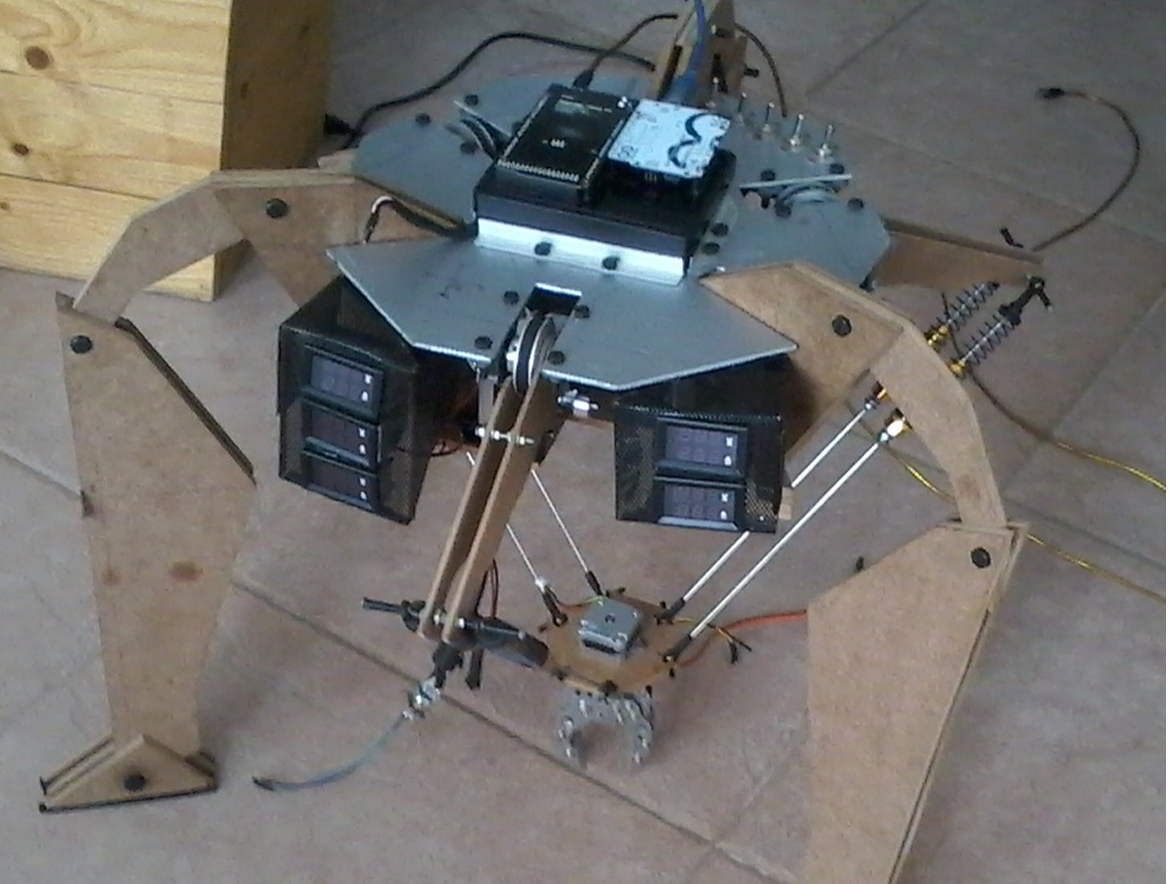
\includegraphics[width=\linewidth,height=1.25in,keepaspectratio]{assets/delta-prototype.png}
\end{minipage}\hfill
\begin{minipage}[b]{0.485\columnwidth}
\centering
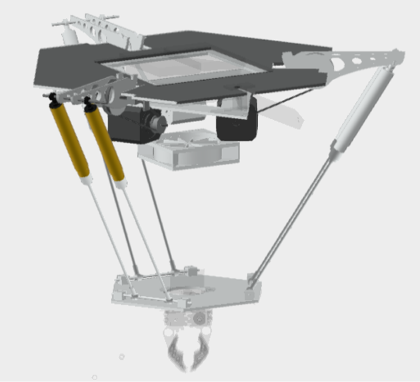
\includegraphics[width=\linewidth,height=1.25in,keepaspectratio]{assets/delta-cad.png}
\end{minipage}
\caption{Constructed Delta prototype (left) and CAD model (right).}
\label{fig:delta}
\end{figure}

Forward kinematics locates the platform through sphere intersection; inverse
kinematics recovers compatible joint angles from a Cartesian target.
Multiple solutions require geometric branch selection. With coordinates
collected in $\mathbf q$, closure constraints $\boldsymbol\Phi$ and their
Jacobian $\mathbf J_\Phi$ satisfy
\begin{equation}
\boldsymbol\Phi(\mathbf q)=\mathbf 0,\qquad
\mathbf J_{\Phi}(\mathbf q)\dot{\mathbf q}=\mathbf 0.
\end{equation}
Differentiation yields configuration-dependent velocity and acceleration
mappings specific to the rigid approximation.

\section{Compliance and Internal States}
The compliant model augments joint coordinates with spring compression
and its time derivative. Lower-member compliance is intended
to soften deceleration loads and isolate end-effector vibration;
compliant supports also maintain transmission tension. Elastic and
viscous forces depend on deformation and its rate, respectively.

The extended representation includes attachment-point geometry and
platform-frame position and orientation. These variables must satisfy
linkage constraints throughout deformation, relating internal motion,
elastic energy, dissipation, and changing force directions to the same
configuration.

\section{Dynamic Formulation and Design Search}
Newtonian joint balances relate actuator input, transmitted torque,
inertia, and gravity under simplifying load assumptions. Appendix~D
outlines a constrained Lagrangian framework for rigid and compliant
representations, combining energy descriptions with geometric
constraints and reaction forces. The explicit control development uses
a reduced dynamic model.

Appendix~C adds a geometric design problem: an evolutionary search varies
link geometry and evaluates approximate reachable workspace volume,
connecting model parameters to a design objective through repeated
kinematic evaluation.

\section{From the Model to Control and Estimation}
Desired Cartesian trajectories are mapped into joint references through
inverse kinematics. Local linearization describes dynamics around the
reference motion; continuous-to-discrete
transformations support a sampled implementation. The analytical
actuator model treats current as the control input under an assumed
inner current-control loop.

Linear-quadratic tracking balances reference error against control
effort. Backward integration of a Riccati equation and a
reference-dependent term determines the feedback and tracking law.
A Luenberger observer reconstructs angular velocity from position
measurements and known control inputs, with estimation-error dynamics
used to choose observer gains. Precomputed matrices and interpolation
reduce the proposed online computation.

\section{Evidence and Model Validation}
The thesis documents prototype construction and presents analytical
tracking responses to smooth and discontinuous references, excluding
the observer. Experimental closed-loop performance remains unverified.
The compliant framework requires completion, parameter identification,
and validation against measured deformation and motion to assess the
model's predictive accuracy.

\bibliographystyle{IEEEtran}
\bibliography{references}
\end{document}
